\section{Experimental Results}
\subsection{Part 1: Hopper}
Figure~\ref{fig:part1-train-comparison} compares REINFORCE without baseline, REINFORCE with a constant baseline of 20, and the actor-critic variant over seeds 0, 42, and 99. All methods improve from the initial policy, but the curves remain noisy, as expected for policy-gradient training on Hopper. The constant baseline gives the strongest final training curve and reduces some early variance relative to plain REINFORCE. The actor-critic variant learns more slowly and reaches lower average returns in this implementation.

\begin{figure}[H]
\centering
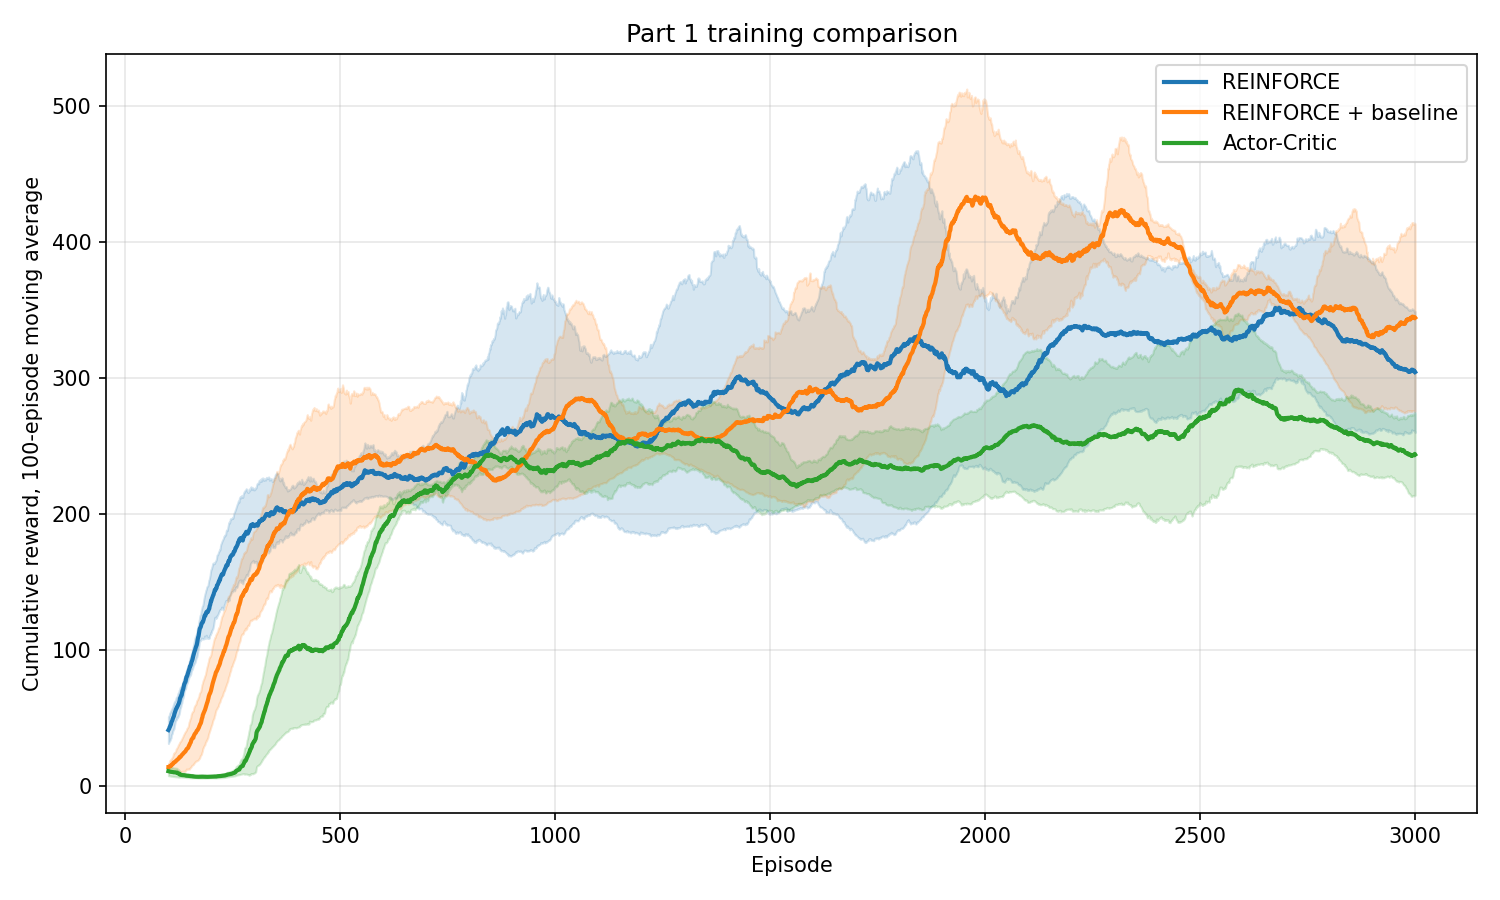
\includegraphics[width=\linewidth]{../part1/plots/comparison_train_mean_std.png}
\caption{Part 1 training comparison on \texttt{Hopper-v4}. Curves show the 100-episode moving average of cumulative reward, averaged over seeds 0, 42, and 99; shaded regions show variability across seeds.}
\label{fig:part1-train-comparison}
\end{figure}

\subsection{Nominal Sim-to-Sim Evaluation}
Table~\ref{tab:nominal-eval} reports deterministic 50-episode evaluations generated from the saved SAC checkpoints. At the nominal target mass of 5 kg, the source-trained SAC policy already transfers well: the gap between source$\rightarrow$source and source$\rightarrow$target is small in success rate.

\begin{table*}[t]
\centering
\small
\begin{tabular}{llccc}
\toprule
Model & Evaluation & Mean return & Std return & Success \\
\midrule
SAC source  & target (easy) & -1.740 & 7.917 & 97.3\%\\
SAC target  & target (easy) & -0.608 & 2.237 & 99.3\% \\
\midrule
SAC source \textbf{(Lower Bound)} & target (hard) & -12.762 & 19.722 & 72.0\% \\
SAC target \textbf{(Upper Bound)} & target (hard) & -6.970 & 16.423 & 85.3\% \\
SAC UDR + friction source & target (hard) & -4.814 & 14.555 & 90.7\% \\
SAC ADR + friction source & target (hard) & -4.638 & 27.440 & 94.0\% \\
\bottomrule
\end{tabular}
\caption{Deterministic SAC evaluations aggregated over 150 episodes, using 50 episodes for each seed in $\{0,42,99\}$. The hard target samples mass from $\mathcal{U}(5,10)$ kg, object/table lateral friction from $\mathcal{U}(0.2,1.5)$, and object spinning friction from $\mathcal{U}(0,0.01)$. The hard target upper-bound checkpoint is not available yet.}
\label{tab:nominal-eval}
\end{table*}

\subsection{Harder Mass and Friction Evaluation}
Because nominal mass transfer was already strong, the evaluation was made harder by randomizing parameters at test time
Table~\ref{tab:nominal-eval} uses mass sampled uniformly in $[5,10]$ kg, object/table lateral friction sampled in $[0.2,1.5]$, and object spinning friction sampled in $[0,0.01]$. Under this harder protocol, the non-randomized source policy drops from 97.3\% to 72\% success on target. The UDR policy trained with mass and friction randomization reaches 90.7\%.
Moreover, the ADR policy generalizes even better on unseen distribution, achieving 94\% of SR on the hard evaluation setting.


\subsection{UDR Hard Target vs.\ ADR Curriculum}

An additional experiment was run to test whether training UDR directly on the target-domain intervals could outperform the ADR curriculum that starts from the source domain.
The \emph{UDR hard target} model was trained with mass sampled from $\mathcal{U}(5,10)$~kg and lateral friction from $\mathcal{U}(0.2,1.5)$, matching the hard evaluation distribution exactly.
Intuitively, this should be the best possible UDR baseline: training and evaluation distributions coincide, so no sim-to-sim gap exists.

Table~\ref{tab:udr-vs-adr} reports deterministic evaluations under the hard target protocol for this model alongside the ADR source model, using 50 episodes for each seed in $\{0,42,99\}$.

\begin{table}[H]
\centering
\small
\begin{tabular}{lccc}
\toprule
Model & Mean return & Std return & Success \\
\midrule
SAC UDR hard target & $-6.970$ & $16.423$ & 85.3\% \\
SAC ADR source      & $-4.638$ & $27.440$ & 94.0\% \\
\bottomrule
\end{tabular}
\caption{Hard target deterministic evaluation aggregated over 150 episodes, using 50 episodes for each seed in $\{0,42,99\}$. Return mean and standard deviation are computed over all episodes. The UDR hard target model was trained with mass $\mathcal{U}(5,10)$~kg and friction $\mathcal{U}(0.2,1.5)$, identical to the evaluation distribution. ADR was trained starting from the source domain with an adaptive curriculum.}
\label{tab:udr-vs-adr}
\end{table}

Despite seeing the same distribution during training and evaluation, the UDR hard target model still performs worse than the ADR curriculum model.
The failure pattern reveals a friction sensitivity: the UDR policy handles low object lateral friction $\mu_\mathrm{obj}\in[0.2,0.5)$ with 100\% success, but its success rate collapses to 55--73\% for medium and high friction values (Table~\ref{tab:udr-friction-bins}).

\begin{table}[H]
\centering
\small
\begin{tabular}{lcc}
\toprule
Object lateral $\mu$ bin & Success (UDR hard) & Success (ADR) \\
\midrule
$[0.21,\,0.46)$ & 100\% & $\approx$100\% \\
$[0.46,\,0.72)$ & 73\%  & $\approx$100\% \\
$[0.72,\,0.97)$ & 55\%  & $\approx$91\%  \\
$[0.97,\,1.22)$ & 71\%  & $\approx$90\%  \\
$[1.22,\,1.48]$ & 64\%  & $\approx$86\%  \\
\bottomrule
\end{tabular}
\caption{Per-friction-bin success rates on the hard target evaluation for the UDR hard target model and the ADR source model (ADR bins are approximate, from the same-seed evaluation).}
\label{tab:udr-friction-bins}
\end{table}


